\documentclass{Beautybook-V6.1-EN}
\coverstyle={
    cover-choose=en, % cn (需新增项\entitle{#}); en ; enfig ; birkar
}
\usepackage{rotating}
\tikzset{>=Stealth}
\setlist{nosep,font=\upshape} % 取消所有列表默认距离
% 浮动环境设置
% 默认情况下, \LaTeX{} 要求每页的文字至少占据 20%,否则该页就只单独放置一个浮动环境,
% 而这通常不是我们想要的, 我们将这个要求降低到 5%.
\renewcommand*{\textfraction}{0.05}
% 有时如果多个浮动环境连续放在一起,
% 会将它们分在几个不同页,即使它们可在同一页放
% 得下. 我们可以通过修改 |\topfraction| 和 |\bottomfraction| 分别设置顶端和底端的浮
% 动环境的最大比例.
\renewcommand*{\topfraction}{0.9}
\renewcommand*{\bottomfraction}{0.8}
% 有时\LaTeX{}会把一个浮动环境单独放在一页,
% 我们要求这个环境至少要占据 85% 才能单独放在一页.
% 注意:  |\floatpagefraction| 的数值必须小于 |\topfraction|.
\renewcommand*{\floatpagefraction}{0.85}
% 关于图片 graphicx
% 如果图片没有指定后缀, 依次按下列顺序搜索
\DeclareGraphicsExtensions{.pdf,.eps,.jpg,.png}
% 设置图表搜索路径, 可以给图表文件夹取如下名字
\graphicspath{{figures/}{figure/}{pictures/}{picture/}{pic/}{pics/}{image/}{images/}}
\usepackage{mtpro2}
\usepackage[physics]{stys/physicx}
\usepackage{stys/Symbols}
\usepackage{amsfonts}
\DeclareFontFamily{U}{nxlmi}{}
\DeclareFontSubstitution{U}{nxlmi}{m}{it}
\DeclareFontShape{U}{nxlmi}{m}{it}{
    <-6.3>    nxlmi05
    <6.3-8.6> nxlmi07
    <8.6->    nxlmi0
}{}

\DeclareFontShape{U}{nxlmi}{b}{it}{
    <-6.3>    nxlbmi05
    <6.3-8.6> nxlbmi07
    <8.6->    nxlbmi0
}{}

\renewcommand{\partial}{{\text{\usefont{U}{nxlmi}{m}{it}\symbol{64}}\mspace{1mu}}}
%% 定义第一种定理
\mynewtheorem{
    defi={\textbf{Definition}}[section]{interior style={left color=ReD!8,right color=ReD!5!CyaN!50}, borderline west={1.5mm}{0mm}{ReD}},
    thm={\textbf{Theorem}}[section]{interior style={left color=CyaN!80!black!20,right color=CyaN!80!black!15!CyaN!50}, borderline west={1.5mm}{0mm}{CyaN!80!black}},
    lem={\textbf{Lemma}}[section]{interior style={left color=BluE!8,right color=BluE!5!CyaN!50}, borderline west={1.5mm}{0mm}{BluE}},
    prop={\textbf{Proposition}}[section]{interior style={left color=OrangE!8,right color=OrangE!5!CyaN!50}, borderline west={1.5mm}{0mm}{OrangE}},
    exam={\textbf{Example}}[chapter]{interior style={left color=DarkGreen!8,right color=DarkGreen!5!CyaN!50}, borderline west={1.5mm}{0mm}{DarkGreen}},
    cor={\textbf{Corollary}}[chapter]{interior style={left color=violet!8,right color=violet!5!CyaN!50}, borderline west={1.5mm}{0mm}{violet}},
}
\newtheorem*{remark}{\textbf{Remark}}
%% 定义第二种定理
%%  用法
% % theorem 环境
% overlay unbroken=\my@theorem@overlay@unbroken{\theorem@name\ \thetcbthm}{额外的选项}
% overlay first=\my@theorem@overlay@first{\theorem@name\ \thetcbthm}{额外的选项}
% % lemma 环境
% overlay unbroken=\my@theorem@overlay@unbroken{\lemma@name\ \thetcblemma}{额外的选项}
%% 用户接口区
\makeatletter
\mynewtcbtheorem{
    % 这个 theorem 是环境名
    theorem={
        counter=tcbthm, 
        the counter=\thesection.\arabic{tcbthm}, 
        name=Theorem, % 它保存到 \theorem@name 里
        thmcolor=高粱红,
        autoref name=\bfseries Theorem, 
        style={
        arc=3pt,breakable,enhanced,interior style={top color=高粱红!12 ,middle color=高粱红!9, bottom color=高粱红!6},boxrule=0pt,top=8mm,
        fuzzy shadow={-0.6mm}{0.6mm}{0mm}{0.3mm}{white!50!gray},% 上
        fuzzy shadow={0.6mm}{-0.6mm}{0mm}{0.3mm}{fill=white!40!gray},%下
        opacityframe=0, opacityback=0.98,
        fontupper=\itshape, step={tcbthm},
        before pre=\smallskip, after app=\smallskip,
        overlay unbroken=\my@theorem@overlay@unbroken{\theorem@name\ \thetcbthm}{\theorem@thmcolor},
        overlay first=\my@theorem@overlay@first{\theorem@name\ \thetcbthm}{\theorem@thmcolor},
        overlay last=\my@theorem@overlay@last,
        }
    },
    proposition={
        counter=tcbprop, 
        the counter=\thesection.\arabic{tcbprop}, 
        autoref name=\bfseries Proposition, 
        style={
        arc=3pt,breakable,enhanced,interior style={top color=高粱红!12 ,middle color=高粱红!9, bottom color=高粱红!6},boxrule=0pt,top=8mm,
        fuzzy shadow={-0.6mm}{0.6mm}{0mm}{0.3mm}{white!50!gray},% 上
        fuzzy shadow={0.6mm}{-0.6mm}{0mm}{0.3mm}{fill=white!40!gray},%下
        opacityframe=0, opacityback=0.98,
        fontupper=\itshape, step={tcbprop},
        before pre=\smallskip, after app=\smallskip,
        overlay unbroken=\my@theorem@overlay@unbroken{Proposition\ \thetcbprop}{高粱红},
        overlay first=\my@theorem@overlay@first{Proposition\ \thetcbprop}{高粱红},
        overlay last=\my@theorem@overlay@last{高粱红},
        }
    },
    definition={
        counter=tcbdefi, 
        the counter=\thesection.\arabic{tcbdefi}, 
        autoref name=\bfseries Definition, 
        style={
        arc=3pt,breakable,enhanced,interior style={top color=紫棠!12 ,middle color=紫棠!9, bottom color=紫棠!6},boxrule=0pt,top=8mm,
        fuzzy shadow={-0.6mm}{0.6mm}{0mm}{0.3mm}{white!50!gray},% 上
        fuzzy shadow={0.6mm}{-0.6mm}{0mm}{0.3mm}{fill=white!40!gray},%下
        opacityframe=0, opacityback=0.98,
        fontupper=\itshape, step={tcbdefi},
        before pre=\smallskip, after app=\smallskip,
        overlay unbroken=\my@theorem@overlay@unbroken{Definition\ \thetcbdefi}{紫棠},
        overlay first=\my@theorem@overlay@first{Definition\ \thetcbdefi}{紫棠},
        overlay last=\my@theorem@overlay@last{紫棠},
        }
    },
    lemma={
        counter=tcblem,
        the counter=\thesection.\arabic{tcblem},
        name=Lemma, 
        lemcolor=靛蓝, 
        autoref name=\bfseries Lemma,
        style={
        arc=0mm,breakable,enhanced,interior style={top color=靛蓝!12 ,middle color=靛蓝!9, bottom color=靛蓝!6},arc=3pt,boxrule=0pt,top=7mm,bottom=5mm,
        fuzzy shadow={-0.6mm}{0.6mm}{0mm}{0.3mm}{white!50!gray},% 上
        fuzzy shadow={0.6mm}{-0.6mm}{0mm}{0.3mm}{fill=white!40!gray},%下
        opacityframe=0, opacityback=0.98,
        fontupper=\normalsize,step={tcblem},
        before pre=\smallskip, after app=\smallskip,
        overlay unbroken=\my@lemma@overlay@unbroken{\lemma@name\ \thetcblem}{\lemma@lemcolor},
        overlay first=\my@lemma@overlay@first{\lemma@name\ \thetcblem}{\lemma@lemcolor},
        overlay last=\my@lemma@overlay@last{\lemma@lemcolor},
        }
    },
    corollary={
        counter=tcbcor,
        the counter=\thesection.\arabic{tcbcor},
        autoref name=\bfseries Corollary,
        style={
        arc=0mm,breakable,enhanced,interior style={top color=茶色!12 ,middle color=茶色!9, bottom color=茶色!6},arc=3pt,boxrule=0pt,top=7mm,bottom=5mm,
        fuzzy shadow={-0.6mm}{0.6mm}{0mm}{0.3mm}{white!50!gray},% 上
        fuzzy shadow={0.6mm}{-0.6mm}{0mm}{0.3mm}{fill=white!40!gray},%下
        opacityframe=0, opacityback=0.98,
        fontupper=\normalsize,step={tcbcor},
        before pre=\smallskip, after app=\smallskip,
        overlay unbroken=\my@lemma@overlay@unbroken{Corollary\ \thetcbcor}{茶色},
        overlay first=\my@lemma@overlay@first{Corollary\ \thetcbcor}{茶色},
        overlay last=\my@lemma@overlay@last{茶色},
        }
    },
    example={
        counter=tcbexam,
        the counter=\thesection.\arabic{tcbexam},
        autoref name=\bfseries Example,
        style={
        arc=0mm,breakable,enhanced,interior style={top color=黛绿!12 ,middle color=黛绿!9, bottom color=黛绿!6},arc=3pt,boxrule=0pt,top=7mm,bottom=5mm,
        fuzzy shadow={-0.6mm}{0.6mm}{0mm}{0.3mm}{white!50!gray},% 上
        fuzzy shadow={0.6mm}{-0.6mm}{0mm}{0.3mm}{fill=white!40!gray},%下
        opacityframe=0, opacityback=0.98,
        fontupper=\normalsize,step={tcbexam},
        before pre=\smallskip, after app=\smallskip,
        overlay unbroken=\my@lemma@overlay@unbroken{Example\ \thetcbexam}{黛绿},
        overlay first=\my@lemma@overlay@first{Example\ \thetcbexam}{黛绿},
        overlay last=\my@lemma@overlay@last{黛绿},
        }
    },
    Exercise={
        counter=tcbexer,
        the counter=\thechapter.\arabic{tcbexer},
        autoref name=\bfseries Exercise,
        style={
        arc=0mm,breakable,enhanced,interior style={top color=绛紫!12 ,middle color=绛紫!9, bottom color=绛紫!6},arc=3pt,boxrule=0pt,top=7mm,bottom=5mm,
        fuzzy shadow={-0.6mm}{0.6mm}{0mm}{0.3mm}{white!50!gray},% 上
        fuzzy shadow={0.6mm}{-0.6mm}{0mm}{0.3mm}{fill=white!40!gray},%下
        opacityframe=0, opacityback=0.9,
        fontupper=\normalsize,step={tcbexer},
        before pre=\smallskip, after app=\smallskip,
        overlay unbroken=\my@lemma@overlay@unbroken{Exercise\ \thetcbexer}{绛紫},
        overlay first=\my@lemma@overlay@first{Exercise\ \thetcbexer}{绛紫},
        overlay last=\my@lemma@overlay@last{绛紫},
        }
    },
}
\makeatother
%

\setsansfont{Arial}
\newenvironment{note}[1][\bf Note:]{\par\Line\uuline{#1} }{\par\Line}
\renewcommand{\Line}{\noindent\tikz\draw[line width=0.65pt,gray!80,dashed] (0,0)--++(.99\linewidth,0);\par}
\newcommand{\Wedge}[1][]{\tikz\path [draw,line width=1pt] (0,0)--++(4pt,12pt) node[right,font=\scriptsize] {#1} --++(4pt,-12pt);}
\newenvironment{key}[1]{\begin{fancybox}{#1}\ }{\end{fancybox}}
\newcommand{\pr}{^\prime}
\newcommand{\prr}{^{\prime\prime}}
\newcommand{\itbf}[1]{\textit{\textbf{#1}}}
\begin{document}
\thispagestyle{empty}
\title{An Introduction to Complex Geometry}
\subtitle{}
\edition{First Edition}
\bookseries{UniversiText}
\author{Ethan Lu}
\pressname{Springer}
\presslogo{inner_pics/Springer-logo.png}
\coverimage{inner_pics/ivy-ge998908f8_1280.jpg}
\makecover

\definecolor{bg}{HTML}{e0e0e0}
\definecolor{fg}{HTML}{455a64}
\colorlet{outermarginbgcolor}{bg}
\colorlet{outermarginfgcolor}{fg}
\colorlet{framegolden}{fg}
\colorlet{framegray}{bg!50}

\thispagestyle{empty}
\begin{titlepage}
\thispagestyle{empty}
    \begin{center}
    
    %% Print the bookseries
    {\makeatletter
    \ifdefvoid{\@bookseries}{}{\bigskip\normalfont\fontsize{20}{20}\selectfont\@bookseries}
    \makeatother}

        \bigskip
        \bigskip

    %% Print the title
    {\makeatletter
    \fontsize{35}{35}\rmfamily\bfseries\selectfont\@title
    \makeatother}
    
    \bigskip
    \bigskip
    
    \bigskip
    \bigskip
    \bigskip

    %% Print the name of the author
    {\makeatletter
    \fontsize{25}{25}\rmfamily\selectfont\@author
    \makeatother}
    
    \bigskip
    \bigskip

    
    \vfill
    
    
    \bigskip
    \bigskip
    
    {\makeatletter
    \fontsize{25}{25}\rmfamily\selectfont\@pressname
    \makeatother}
    \end{center}
    
    \end{titlepage}
    \let\cleardoublepage\clearpage

    \thispagestyle{empty}
    \begin{center}
        {\fontsize{20}{20}\rmfamily\selectfont    Simple Introduction}\\ 
        \bigskip
        This book is my notes of Complex Geometry!
        \bigskip
        
        This book is a summary of the final examination review materials of complex analysis, mainly including the proof question types of the exam and various knowledge points, such as Riemann mapping theorem, generalized Schwarz lemma and so on. This book was written by me at the end of the semester and is for review only.

        \bigskip

        {\fontsize{10}{10}\rmfamily\bfseries\selectfont Cataloging books in Print (CIP) data}\\[-2ex]
        \tikz\draw[line width=1pt,black] (0,0)-- (.99\linewidth,0);\\[-.8ex]
        Complex Geometry Notes/(en) Etan Lu --Guangdong; xx press,2023.01 \\ 
        (\@bookseries)\\ 
        {\bfseries ISBN: } 978-7-03-002970-6\\ 
        I.xx......\circled{1} Ethan......\\ 
        CIP data kernel word of China Edition Library(2023) The 00022893 number \\[-2ex]
        \tikz\draw[line width=1pt,black] (0,0)-- (.99\linewidth,0);\\[-.8ex]
        {\itshape editor in charge: Ethan Lu / Responsibility proofreading: Ethan Lu\\ 
        Responsibility printing: Ehtan Lu}
        \vfill

        {\makeatletter
    \fontsize{10}{10}\rmfamily\selectfont\@pressname 
    \makeatother}publish\\ 
    {\footnotesize 290 Xinyi City, Maoming City, Guangdong Province}\\ 
    \href{https://www.lushilong.com}{Etan Lu}\\ 
    {\fontsize{10}{10}\rmfamily\selectfont Guangdong Printing Co. LTD} painting\\ 
    xx press\hspace{2em} Xinhua bookstore distribution around\\ 
    \bigskip
    *\\
    \bigskip
    {\footnotesize\begin{tabular}{ll} 2023-02 version I & page: $850\times1168\quad \quad1/32$\\ 
    2023-05 version II & number: $18 5/8$\\ 
    \multicolumn{2}{c}{words:493 000}\\
    \end{tabular}}\\ 
    {\fontsize{10}{10}\rmfamily\bfseries\selectfont price: 89.00}\\ 
    {\footnotesize (If there is any printing problem, we will replace it)}


    \end{center}






\frontmatter
\pagenumbering{Roman}
\thispagestyle{empty}
\addcontentsline{toc}{chapter}{Preface}
\chapter*{Preface}
As my first english book, i'm happy.

\hfill
\begin{tabular}{lr}
    &----- Ethan Lu\\ 
    &2023-01-11
\end{tabular}

\let\cleardoublepage\clearpage

\thispagestyle{empty}
\tableofcontents\let\cleardoublepage\clearpage


\mainmatter
\pagenumbering{arabic}

\partimage{inner_pics/part.png}
\partabstract{A small introduction A small introduction A small introduction A small introduction A small introduction A small introduction}
\part{Exercises Of Riemannian Geometry (Ver : Do Carmo)}
\newcommand*{\x}{\mathbf{x}}
\newcommand*{\y}{\mathbf{y}}
\newcommand*{\z}{\mathbf{z}}
\chapter{Differentiable Manifolds}
\section{Exercises 0}
\begin{proposition}[][Proposition A.17 (Properties of the Subspace Topology).]
    Let $X$ be a topological space and let $S$ be a subspace of $X$.\cite{Huybrechts2010Complex}
    \begin{enumerate}[label=(\alph*)]
        \item {\color{靛蓝}\textsc{Characteristic Property}: If $Y$ is a topological space, a map $F: Y \rightarrow S$ is continuous if and only if the composition  $\iota_S \circ F: Y \rightarrow X$ is continuous, where $\iota_S: S \hookrightarrow X$ is the inclusion map (the restriction of the identity map of $X$ to $S$ ).}
        \item The subspace topology is the unique topology on $S$ for which the characteristic property holds.
        \item A subset $K \subseteq S$ is closed in $S$ if and only if there exists a closed subset $L \subseteq X$ such that $K=L \cap S$.
        \item The inclusion map $\iota_S: S \hookrightarrow X$ is a topological embedding.
        \item If $Y$ is a topological space and $F: X \rightarrow Y$ is continuous, then $\left.F\right|_S: S \rightarrow Y$ (the restriction of $F$ to $S$ ) is continuous.
        \item If $\mathscr{B}$ is a basis for the topology of $X$, then $\mathscr{B}_S=\{B \cap S: B \in \mathscr{B}\}$ is a basis for the subspace topology on $S$.
        \item If $X$ is Hausdorff, then so is $S$.
        \item If $X$ is first-countable, then so is $S$.
        \item If $X$ is second-countable, then so is $S$.
    \end{enumerate}
\end{proposition}
\begin{proposition}[][Proposition A.23 (Properties of the Product Topology).]
    Suppose $X_1, \ldots, X_k$ are topological spaces, and let $X_1 \times \cdots \times X_k$ be their product space.
    \begin{enumerate}[label=(\alph*)]
    \item {\color{靛蓝}\textsc{Characteristic Property}: If $B$ is a topological space, a map $F: B \rightarrow$ $X_1 \times \cdots \times X_k$ is continuous if and only if each of its component functions $F_i=$ $\pi_i \circ F: B \rightarrow X_i$ is continuous.}
    \item The product topology is the unique topology on $X_1 \times \cdots \times X_k$ for which the characteristic property holds.
    \item Each projection map $\pi_i: X_1 \times \cdots \times X_k \rightarrow X_i$ is continuous.
    \item Given any continuous maps $F_i: X_i \rightarrow Y_i$ for $i=1, \ldots, k$, the product map $F_1 \times \cdots \times F_k: X_1 \times \cdots \times X_k \rightarrow Y_1 \times \cdots \times Y_k$ is continuous, where
    \begin{align*}
    F_1 \times \cdots \times F_k\left(x_1, \ldots, x_k\right)=\left(F_1\left(x_1\right), \ldots, F_k\left(x_k\right)\right) .
    \end{align*}
    \item If $S_i$ is a subspace of $X_i$ for $i=1, \ldots, n$, the product topology and the subspace topology on $S_1 \times \cdots \times S_n \subseteq X_1 \times \cdots \times X_n$ coincide.
    \item For any $i \in\{1, \ldots, k\}$ and any choices of points $a_j \in X_j$ for $j \neq i$, the map $x \mapsto\left(a_1, \ldots, a_{i-1}, x, a_{i+1}, \ldots, a_k\right)$ is a topological embedding of $X_i$ into the product space $X_1 \times \cdots \times X_k$.
    \item If $\mathscr{B}_i$ is a basis for the topology of $X_i$ for $i=1, \ldots, k$, then the collection
    \begin{align*}
    \mathscr{B}=\left\{B_1 \times \cdots \times B_k: B_i \in \mathscr{B}_i\right\}
    \end{align*}
    is a basis for the topology of $X_1 \times \cdots \times X_k$.
    \item Every finite product of Hausdorff spaces is Hausdorff.
    \item Every finite product of first-countable spaces is first-countable.
    \item Every finite product of second-countable spaces is second-countable.
\end{enumerate}
\end{proposition}
\begin{example}[][Example 1.8 (Product Manifolds).][Exam:1.8]
    Suppose $M_1, \ldots, M_k$ are topological manifolds of dimensions $n_1, \ldots, n_k$, respectively. The product space $M_1 \times \cdots \times M_k$ is shown to be a topological manifold of dimension $n_1+\cdots+n_k$ as follows. \textbf{\itshape It is Hausdorff and second-countable by Propositions A.17 (g), (i) and A.23 (h), (j), so only the locally Euclidean property needs to be checked.} Given any point $\left(p_1, \ldots, p_k\right) \in$ $M_1 \times \cdots \times M_k$, we can choose a coordinate chart $\left(U_i, \varphi_i\right)$ for each $M_i$ with $p_i \in U_i$. {\bf\itshape The product map
\begin{align*}
\varphi_1 \times \cdots \times \varphi_k: U_1 \times \cdots \times U_k \rightarrow \mathbb{R}^{n_1+\cdots+n_k}
\end{align*}
is a homeomorphism onto its image, which is a product open subset of $\mathbb{R}^{n_1+\cdots+n_k}$.} Thus, $M_1 \times \cdots \times M_k$ is a topological manifold of dimension $n_1+\cdots+n_k$, with charts of the form $\left(U_1 \times \cdots \times U_k, \varphi_1 \times \cdots \times \varphi_k\right)$.

\end{example}
\begin{example}[][Example 1.9 (Tori).]
    For a positive integer $n$, the $\boldsymbol{n}$-torus (plural: tori) is the product space $\mathbb{T}^n=\mathbb{S}^1 \times \cdots \times \mathbb{S}^1$. By the discussion above, it is a topological $n$-manifold. (The 2-torus is usually called simply the torus.)
\end{example}
\begin{example}[][Example 1.34 (Smooth Product Manifolds).][Exam:1.34]
    If $M_1, \ldots, M_k$ are smooth manifolds of dimensions $n_1, \ldots, n_k$, respectively, we showed in \autoref{Exam:1.8} that the product space $M_1 \times \cdots \times M_k$ is a topological manifold of dimension $n_1+\cdots+n_k$, with charts of the form $\left(U_1 \times \cdots \times U_k, \varphi_1 \times \cdots \times \varphi_k\right)$. {\bf\itshape Any two such charts are smoothly compatible because, as is easily verified,
    \begin{align*}
    \left(\psi_1 \times \cdots \times \psi_k\right) \circ\left(\varphi_1 \times \cdots \times \varphi_k\right)^{-1}=\left(\psi_1 \circ \varphi_1^{-1}\right) \times \cdots \times\left(\psi_k \circ \varphi_k^{-1}\right),
    \end{align*}
    which is a smooth map.} This defines a natural smooth manifold structure on the product, called the product smooth manifold structure. For example, this yields a smooth manifold structure on the $n$-torus $\mathbb{T}^n=\mathbb{S}^1 \times \cdots \times \mathbb{S}^1$.
\end{example}
\begin{Exercise}[][Product Manifold]
    Let $M$ and $N$ be differentiable manifolds and let $\{(U_\alpha,\x_\alpha)\}, \{(V_\alpha,\y_\alpha)\}$ be differentiable structure on $M$ and $N$, respectively. Consider the cartesian product $M\times N$ and the mappings $\z_{\alpha\beta}(p,q)=(\x_\alpha (p),\y_\beta (q)), p\in U_\alpha, q\in V_\beta$.
    \begin{enumerate}[label=(\bf\alph*)]
        \item Prove that $\{(U_{\alpha\beta},\z_{\alpha\beta})\}$ is a differentiable structure on $M\times N$ in which the projections $\pi_1\colon M\times N \to M$  and $\pi_2\colon M\times N \to N$ are differentiable. With this differentiable structure $M\times N$ is called the product manifold of $M$ with $N$.
        \item Show that the product manifold $S^1\times \cdots\times S^1$ of $n$ circles $S^1$, where $S^1\subset \bR^2$ has the usual differentiable structure , is diffeomorphic to the $n$ torus $T^n$ of \textsf{Example 4.9 (a)}.
    \end{enumerate}
\end{Exercise}
\begin{proof}
For (a), \begin{enumerate}
    \item (Open Covering) As 
    \begin{align*}
        \z_{\alpha\beta} \colon & U_\alpha\times V_\beta \to \x_\alpha (U_\alpha)\times \y_{\beta}(V_\beta)\subset M\times N\\ 
        &(p,q) \mapsto (\x_\alpha(p),\y_\beta(q))
    \end{align*}
        is a homeomorphism, there is a open covering of $M\times N$ , i.e. 
        \[\bigcup_{\alpha,\beta}\z_{\alpha\beta}(U_\alpha,V_\beta)=\bigcup_\alpha \x_\alpha (U_\alpha)\times \bigcup_\beta \y_\beta (V_\beta)=M\times N.\]
    \item (Atlas Compatibility) When $\z_{\alpha\beta}(U_\alpha,V_\beta)\bigcap \z_{\gamma\delta}(U_\gamma,V_\delta)\neq \emptyset$, one has 
    \[\z_{\gamma\delta}^{-1}\circ \z_{\alpha\beta} (p,q)=\z_{\gamma\delta}^{-1}(\x_\alpha(p),\y_\beta(q))=(\x_\gamma^{-1}\circ \x_\alpha(p),\y_\delta^{-1}\circ \y_\beta(q))\]
    is differentiable, i.e. any two charts of atlas are compatible.
\end{enumerate}
Thus, by definition, with this differentiable structure, $M\times N$ is a differentiable manifold.

For (b), define a mapping
\begin{align*}
\begin{aligned}
& \varphi: \mathbb{R}^n / G \rightarrow \overbrace{\mathbb{S}^1 \times \ldots \times \mathbb{S}^1}^{\mathrm{n} \text { copies }} \\
& \left(x_1, \ldots, x_n\right) \mapsto\left(e^{2 \pi i \frac{x_1}{m_1}}, \ldots, e^{2 \pi i \frac{x_n}{m_n}}\right)
\end{aligned}
\end{align*}
It is obviously that $\varphi$ is an immersion and submersion from its Jacobi matrix:
\begin{align*}
J(\varphi)=\left(\begin{array}{ccc}
\frac{2 \pi i}{m_1} e^{2 \pi i \frac{x_1}{m_1}} & \\
& \ddots & \\
& & \frac{2 \pi i}{m_n} e^{2 \pi i \frac{x_n}{m_n}}
\end{array}\right)
\end{align*}
So $\varphi$ is diffeomorphism.
\end{proof}

\begin{Exercise}
    Prove that the tangent bundle of a differentiable manifold $M$ is orientable (even though $M$ may be not).
\end{Exercise}
\begin{proof}
    Choose a parametrization $\left\{\left( U_\alpha, X_\alpha\right)\right\}$ of M. it induce a parametrization of TM:
\begin{align*}
\begin{aligned}
 Y_\alpha : & U_\alpha \times\mathbb{R}^n \rightarrow \pi^{-1}\left(X_\alpha\left(U_\alpha\right)\right)\subset \textrm{TM} \\
& (x, t) \mapsto\left(X_\alpha(x), d X_\alpha(t)\right)
\end{aligned}
\end{align*}

The corresponding coodinate transformation is
\begin{align*}
Y_\beta^{-1} Y_\alpha(x, t)=\left(X_\beta^{-1} X_\alpha(x), d X_\beta^{-1} d X_\alpha(t)\right)=\left(X_\beta^{-1} X_\alpha(x), d\left(X_\beta^{-1} X_\alpha\right)(t)\right)
\end{align*}
To calculate its Jacobi matrix, we get
\begin{align*}
J\left(Y_\beta^{-1} Y_\alpha\right)=\left[\begin{array}{cc}
J & O \\
* & J
\end{array}\right], \quad J=J\left(X_\beta^{-1} X_\alpha\right)
\end{align*}
And its determination
\begin{align*}
\operatorname{det} J\left(Y_\beta^{-1} Y_\alpha\right)=(\operatorname{det} J)^2>0
\end{align*}
So, TM is an orientable manifold.
\end{proof}

\begin{Exercise}
    Prove that:
    \begin{enumerate}[label=(\alph*)]
        \item A regular surface $S \subset \mathbb{R}^3$ is an orientable manifold if and only if there exists a differentiable mapping of $N: S \rightarrow \mathbb{R}^3$ with $N_p \perp T_p S,\left|N(p)\right|=1, \forall p \in S$,
        \item the M\"{o}bius band (Example 4.9 (b)) is non--orientable.
    \end{enumerate}
\end{Exercise}

\begin{proof}
    \begin{enumerate}[label=(\alph*)]
        \item $(\Rightarrow)$ Choose a parametrization $\left\{\left(X_\alpha, U_\alpha\right)\right\}$ of $S$. For any points $p \in X_\alpha\left(U_\alpha\right) \cap X_\beta\left(U_\beta\right) \subset S$, which $p=X_\alpha\left(x_1, x_2\right)=X_\beta\left(y_1, y_2\right)$. Since $S$ is an orientable, thus
$\operatorname{det} d\left(X_\beta^{-1} \circ X_\alpha\right)>0, \quad \forall \alpha, \beta$
Define a mapping
\begin{align*}
N(p)=N\left(X_\alpha\left(x_1, x_2\right)\right):=\frac{\frac{\partial}{\partial x_1} \wedge \frac{\partial}{\partial x_2}}{\left|\frac{\partial}{\partial x_1} \wedge \frac{\partial}{\partial x_2}\right|}, \frac{\partial}{\partial x_j} \in T_p S=\mathbb{R}^2 \subset \mathbb{R}^3
\end{align*}
Then
\begin{align*}
N(p)&=N\left(X_\beta\left(y_1, y_2\right)\right)\\
&=\frac{\frac{\partial}{\partial y_1} \wedge \frac{\partial}{\partial y_2}}{\left|\frac{\partial}{\partial y_1} \wedge \frac{\partial}{\partial y_2}\right|}=\frac{\operatorname{det}\left(d\left(X_\beta^{-1} \circ X_\alpha\right)\right)}{\left|\operatorname{det}\left(d\left(X_\beta^{-1} \circ X_\alpha\right)\right)\right|} \cdot \frac{\frac{\partial}{\partial x_1} \wedge \frac{\partial}{\partial x_2}}{\left|\frac{\partial}{\partial x_1} \wedge \frac{\partial}{\partial x_2}\right|}=\frac{\frac{\partial}{\partial x_1} \wedge \frac{\partial}{\partial x_2}}{\left|\frac{\partial}{\partial x_1} \wedge \frac{\partial}{\partial x_2}\right|}
\end{align*}
$N(p)$ is well defined.
$(\Leftarrow)$ Suppose that $N(p)$ is a differentiable mapping as we known.
        \item We say that $\mathrm{M}$ is orientable if and only if there exists an atlas $A=\left\{\left(U_\alpha, \phi_\alpha\right)\right\}$ such that $\operatorname{det}\left(J\left(\phi_\alpha \circ \phi_\beta^{-1}\right)\right)>0$, if it is defined.

        Assume that the M\"obius strip (band) is orientable. Then we would be able to define a map: $x \rightarrow \boldsymbol{n}_{\boldsymbol{x}}$ that sends $x$ to a unit vector normal to the surface in such a way that the map is continuous. Since $M$ is two-dimensional and embedded in 3-space, this map is determined by the value at a single point (because you have two choices, one in each direction from the surface). Now observe that if you follow a loop around the strip, the value of $\boldsymbol{n}_{\boldsymbol{x}}$ changes sign when you return to $\boldsymbol{x}$ from the other side.

        Reference: \href{https://mathinsight.org/moebius_strip_not_orientable}{The M\"obius strip (band) is non-orientable.}
    \end{enumerate}
    
\end{proof}
4.
\begin{proof}
    For simplicity, assume (without loss of generality) that in the following, by "chart" I mean ``connected chart". 
    
    By definition, a manifold $M$ is orientable iff you can find a covering of $M$ by coherently oriented charts. Meaning that the determinant of the derivative of the transition functions between overlapping charts (i.e. $\det(J)$) are all positive. Next, note that given two charts $(U,f), (V,g)$ of $M$ of opposite orientation (i.e. the transition function is of negative determinant), the charts $(U,f^*),(V,g)$ are of the same orientation, where $f^*$ is defined by changing the sign of the first coordinate of $f$. Call $(U,f^*)$ the ``modified" chart $(U,f)$. 
    
    Thirdly, note that a manifold $M$ is orientable iff given any covering of $M$ by charts, it is always possible to modify them (in the above sense) to obtain a coherently oriented covering of $M$. 
    
    $(\Longleftarrow)$ Clearly.
    
    $(\Longrightarrow)$ Let $\{(U_i,f_i)\}$ be any covering of $M$ by charts. Take a coherently oriented covering of $M$ by charts $\{(V_j,g_j)\}$. For each $U_i$, chose a $ V_j $ that intersects it. Are $U_i$ and $V_j$ of the same orientation? If so, do nothing. If not, modify $(U_i,f_i)$ to $(U_i,f^*_i)$. Note that for two charts to have the same orientation is an equivalence relation on the set of all charts of a manifold. Clearly then, this process makes $\{(U_i,f_i)\}$ into a coherently oriented covering.  
    
    Now let $M$ be $2$ dimensional. Let $X=([0,1] x ]-1,1[)/(0,t)~(1,-t)$ be the M\"obius band, and $f:X\longrightarrow M$ be an embedding. Consider $\{(U_i,\phi_i)\}$ a covering of $f(X)$ by charts lying entirely in $f(X)$ ($f(X)$ is open in $M$). Since the ``pullback charts" $(f^{-1}(U_i), \phi_i \circ f)$ make up a covering of the nonorientable manifold $X$, it is impossible to modify the covering $\{(U_i,\phi_i)\}$ to make it coherently oriented. Then just extend $\{(U_i,\phi_i)\}$ to a covering of the whole of $M$. This covering either cannot be modified to be coherently oriented, so $M$ is nonorientable. %QED

Reference: \href{https://www.physicsforums.com/threads/how-to-understand-that-rp2-is-non-orientable.420456/}{$\bR P^n$ is non-orientable.}

\end{proof}
5.
\begin{proof}
    (a) $\tilde{\varphi}: P^2 \rightarrow \mathbb{R}^4$ is a immersion.
Pf: Since
\begin{align*}
d \tilde{\varphi}_{[p]}=d \varphi_p=J_p(F)=\left(\begin{array}{rrrr}
2 x & y & z & 0 \\
-2 y & x & 0 & z \\
0 & 0 & x & y
\end{array}\right)^T
\end{align*}
Let $p=(0,0,1)$ For symmetry of sphere $\mathbb{S}^2$.
\begin{align*}
\Rightarrow J_p(F)=\left(\begin{array}{llll}
0 & 0 & 1 & 0 \\
0 & 0 & 0 & 1 \\
0 & 0 & 0 & 0
\end{array}\right)^T
\end{align*}
$\operatorname{rank} d F_p=\operatorname{dim} T_p \mathbb{S}^2=2$, So $\tilde{\varphi}$ is a immersion.

(b) $\tilde{\varphi}$ is injective; together with (a) and the compactness of $P^2$, this implies that $\tilde{\varphi}$ is an embedding.
Pf: If $\tilde{\varphi}([p])=\tilde{\varphi}([q])$, where $p=(x, y, z), q=\left(x^{\prime}, y^{\prime}, z^{\prime}\right)$, it means
\begin{align*}
\begin{cases}x^2+y^2+z^2=x^{\prime 2}+y^{\prime 2}+z^{\prime 2}=1 \\ x^2-y^2=x^2-y^{\prime 2} \\ x y=x^{\prime} y^{\prime} & (* 1) \\ x z=x^{\prime} z^{\prime} & (* 2) \\ y z=y^{\prime} z^{\prime} & (* 3)\end{cases}
\end{align*}
From $(* 1) \times(* 2)$ we obtained
\begin{align*}
x^2 y z=x^2 y^{\prime} z^{\prime}
\end{align*}
If $y z \neq 0$, by $(* 3)$ we get
\begin{align*}
x= \pm x^{\prime}
\end{align*}
By the continuity of the equations, when $y \rightarrow 0$ or $z \rightarrow 0$, it still holds.
Similarly, we can get $y= \pm y^{\prime}, z= \pm z^{\prime}$. Thus, $p=-q \in[p]$.
\end{proof}

6.
\begin{Exercise}
    Show that the mapping $G\colon \bR^2\to\bR^4$ given by 
    \[G(x,y)=((r\cos y+a)\cos x,(r\cos y+a)\sin x, r\sin y\cos \frac{x}{2},r\sin x\sin \frac{x}{2}), \]
    with $(x,y)\in\bR^2$ induces an embedding of the klein bottle into $\bR^4$.
\end{Exercise}

\begin{proof}
% To show that the mapping $G\colon \bR^2\to\bR^4$ given by 
% \[G(x,y)=((r\cos y+a)\cos x,(r\cos y+a)\sin x, r\sin y\cos \frac{x}{2},r\sin x\sin \frac{x}{2}), (x,y)\in\bR^2\]
% induces an embedding of the Klein bottle into $\bR^4$, we need to show that $G$ is an immersion (i.e. its derivative is injective at every point), and that $G$ is a homeomorphism onto its image.
% First, we compute the derivative of $G$:
% $$
% DG(x,y) = \begin{pmatrix}
% -(r\cos y +a) \sin x & (r\cos y+a)\cos x & -\frac{1}{2}r\sin y \sin \frac{x}{2} & \frac{1}{2}r\cos y\cos \frac{x}{2}\\
% (-r\sin y +a) \cos x & (-r\sin y+a)\sin x &r\cos y\cos \frac{x}{2} & r\cos y\sin \frac{x}{2}\\
% \cos y \cos x & \cos y \sin x &\sin y \cos \frac{x}{2} & \sin y \sin \frac{x}{2}\\
% \cos x & \sin x & 0 & 0
% \end{pmatrix}.
% $$
% The derivative $DG(x,y)$ has rank 4 unless $r=0\text{ or }1$ and $a=0$ (when $r=0$, the mapping degenerates to a point, while when $r=1$ and $a=0$, the mapping corresponds to the usual parametrization of the torus). So $G$ is non-degenerate.

% To show that $G$ is a homeomorphism onto its image, we need to show that $G$ is continuous, injective (so that we can define its inverse), and that the inverse is also continuous. Continuity of $G$ follows from the continuity of its component functions and elementary properties of the trigonometric functions.

% To show that $G$ is injective, we need to show that distinct points in the domain of $G$ are mapped to distinct points in the image of $G$. This follows from the fact that the horizontal and vertical components of $G(x,y)$ depend only on $x$ and $y$ respectively, while the other two components involve both $x$ and $y$ in a nontrivial way.

% To show that the inverse of $G$ is continuous, we need to show that the preimage of any open set in the image of $G$ is open in the domain of $G$. This can be done using the inverse function theorem, which guarantees that $G$ is a local diffeomorphism at every point where $DG$ is invertible.
% Therefore, we have shown that $G$ induces an embedding of the Klein bottle into $\bR^4$.

To show that $G$ induces an embedding of the Klein bottle into $\bR^4$, we need to show that $G$ is an immersion and a homeomorphism onto its image.

First, we will show that $G$ is an immersion. To do this, we need to show that $DG(x,y)$ is injective for all $(x,y) \in \bR^2$. We have already computed the matrix $DG(x,y)$ in the previous answer, so we only need to check that its determinant is nonzero. The derivative of $G$ at $(x,y)\in \bR^2$ is the $4\times 2$ matrix 
$$
DG(x,y) = \begin{pmatrix}
-(r\cos y +a) \sin x & (r\cos y+a)\cos x &a-r\sin y \sin \frac{x}{2} & \frac{1}{2}r\cos x\cos \frac{x}{2}\\
-(r\cos y +a) \cos x &a-(r\cos y+a)\sin x & 0 & \frac{1}{2}r\cos x\sin \frac{x}{2}\\
0 & -r\cos y \cos \frac{x}{2} & -\frac{1}{2}r\sin y\sin \frac{x}{2} & r\sin y\cos \frac{x}{2}\\
0 &-r\sin y\sin \frac{x}{2} & \frac{1}{2}r\sin x\cos \frac{x}{2} & \frac{1}{2}r\sin x\sin \frac{x}{2}
\end{pmatrix}.
$$

Then the determinant of $\det DG(x,y)$ is 
$$
\det DG(x,y) = -\frac{1}{2}r^2\sin^2 x\sin y \neq 0,
$$
\textit{\textbf{ so $DG(x,y)$ is always invertible (i.e. $G$ is non-degenerate). Therefore,  $G$ is an immersion}}.

Next, we will \itbf{ show that $G$ is a homeomorphism onto its image}. To do this, we need to show that \itbf{ $G$ is bijective, continuous, and has a continuous inverse}.

To show that $G$ is bijective, we need to show that distinct points in the domain of $G$ are mapped to distinct points in the image of $G$, and that every point in the image of $G$ is the image of some point in the domain of $G$. 

The first part follows from the fact that the horizontal and vertical components of $G(x,y)$ depend only on $x$ and $y$, respectively, while the other two components involve both $x$ and $y$ in a nontrivial way. Specifically, if $(x1,y1) \neq (x2,y2)$, then there must be at least one component of $G(x1,y1)$ that is different from the corresponding component of $G(x2,y2)$.

The second part follows from the fact that every point on the Klein bottle can be parametrized by $(x,y) \in [0,2\pi) \times [0,2\pi)$, which is precisely the domain of $G$. Therefore, $G$ is bijective.
To show that $G$ is continuous, we need to show that each component of $G$ is a continuous function of $(x,y)$. We can see that this is the case, since each component is a sum and product of trigonometric functions, which are all continuous.

To show that $G^{-1}$ is continuous, we need to show that $G^{-1}(U)$ is open in $\bR^2$ for every open set $U$ in the image of $G$. To do this, we will use the inverse function theorem, which states that if $\det DG(x,y) \neq 0$ for all $(x,y) \in U$, then $G$ is a local diffeomorphism on $U$ and $G^{-1}$ is continuous on $G(U)$. By our earlier computation, we know that $\det DG(x,y) \neq 0$ for all $(x,y) \in \bR^2$, so we don't need to worry about singular points.

Therefore, we have shown that $G$ induces an embedding of the Klein bottle into $\bR^4$.
\end{proof}
7.
\begin{proof}
    
\end{proof}
8. 
\begin{proof}
\begin{figure}[htbp]
    \centering
    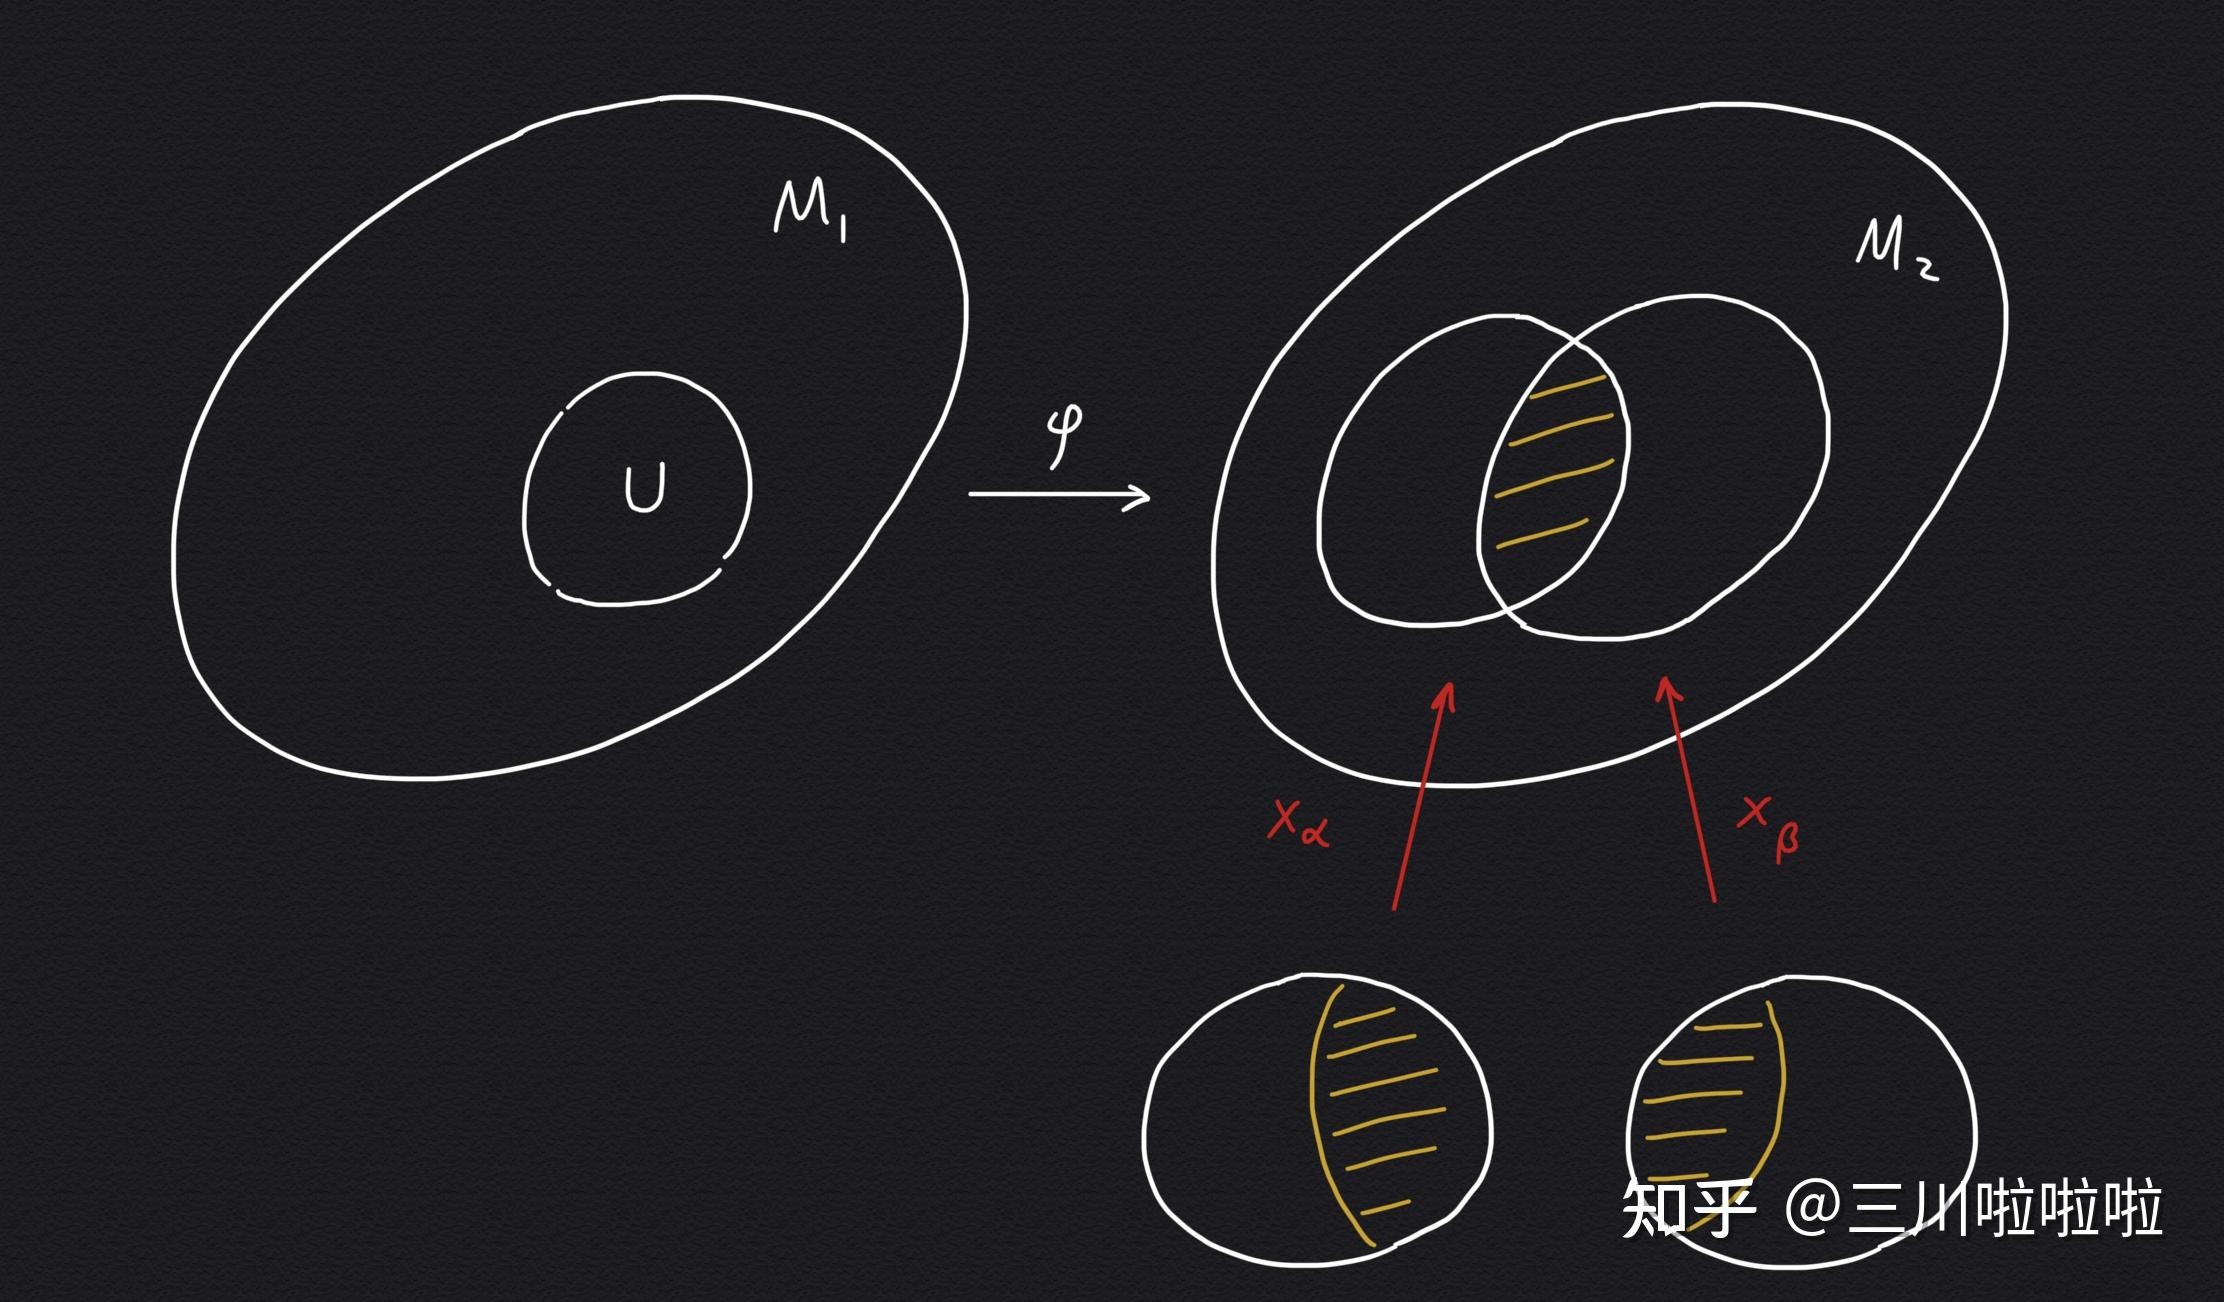
\includegraphics[width=.5\linewidth]{figures/ex8.jpg}
    \caption{exercise 8}
    \label{fig:ex8}
\end{figure}
    Pf: Let $\varphi: U \subset M_1 \rightarrow \varphi(U) \subset V_\alpha \cap V_\beta \subset M_2, V_\alpha, V_\beta$ are charts of $M_2$. Since $\varphi$ is a local diffeomorphisma, $\left\{\varphi^{-1}\left(U \cap X_\alpha\left(V_\alpha\right)\right), X_\alpha \circ \varphi\right\}$ is a parametrization of $M_1$. Since $M_2$ is orientable, i.e. $\operatorname{det}\left(d\left(X_\beta^{-1} \circ X_\alpha\right)\right)>0$. Therefore, for $p \in\left(U_1 \cap X_\alpha\left(V_\alpha\right)\right) \cap\left(U_2 \cap X_\beta\left(V_\beta\right)\right) \neq \varnothing$
\begin{align*}
\operatorname{det}\left(d\left(\left(X_\beta \circ \varphi\right)^{-1} \circ X_\alpha \circ \varphi\right)\right)=\operatorname{det}\left(d\left(\varphi^{-1} X_\beta^{-1} \circ X_\alpha \circ \varphi\right)\right)=\operatorname{det}\left(d\left(X_\beta^{-1} \circ X_\alpha\right)\right)>0 .
\end{align*}
\end{proof}


\begin{Exercise}[][Exer 9.]
    Let $G \times M \rightarrow M$ be a properly discontinuous action of a group $G$ on a differentiable manifold $M$.

a) Prove that the manifold $M / G$ (Example 4.8) is oriented if and only if there exists an orientation of $M$ that is preserved by all the diffeomorphisms of $G$.

b) Use a) to show that the projective plane $P^2(\mathbb{R})$, the Klein bottle and the Mobius band are non-orientable.

c) Prove that $P^2(\mathbb{R})$ is orientable if and only if $n$ is odd.
\end{Exercise}
\begin{proof}
 a) if part: Let $\left(U_\alpha, x_\alpha\right)$ be an orientation of $\mathrm{M}$ that is preserved by all the diffeomorphisms of $G$, i.e.
\begin{align*}
W=U_\beta \cap g\left(U_\alpha\right) \neq \varnothing \Rightarrow \operatorname{det}\left(x_\beta^{-1} \circ g \circ x_\alpha\right)>0
\end{align*}
We claim that $\left(\pi\left(U_\alpha\right), \pi \circ x_\alpha\right)$ is an orientation of $M / G$. Indeed,
\begin{align*}
\pi\left(U_\alpha\right) \cap \pi\left(U_\beta\right) \neq \varnothing \Rightarrow \operatorname{det}\left(\left(\pi \circ x_\beta\right)^{-1} \circ\left(\pi \circ x_\alpha\right)\right)=\operatorname{det}\left(x_\beta^{-1} \circ g \circ x_\alpha\right)>0
\end{align*}
for some $g \in G$.
Only if part: We know the atlas of $M / G$ is induced from $M$, hence the conclusion follows from the reverse of the "if part".

b) Let $G=\{I d, A\}$ where $A$ is the antipodal map. Recall that
\begin{align*}
    \text{Projective $2-$ space $P^2(\mathbb{R})=S^2 / G$, where $S^2$} =2-\operatorname{dim} \text{sphere}\\
\text{Klein bottle $K=\mathbb{T}^2 / G$, where $\mathbb{T}^2$}=2-\operatorname{dim} \text{torus}\\
\text{Mobius band $M=C / G$, where $C$}=2-\operatorname{dim} \text{cylinder}
\end{align*}


Clearly, $S^2, \mathbb{T}^2, C$ are orientable $2-\operatorname{dim}$ manifols, but $A$ reverse the orientation of $\mathbb{R}^3$, hence $S^2, \mathbb{T}^2, C$. The conclusion follows from a).

c) We've the following equivalence:
\begin{align*}
\begin{aligned}
& P^n(\mathbb{R}) \text { is orientable } \Leftrightarrow A \text { preserves the orientation of } S^n(\text { by } a) \text { ) } \\
& \Leftrightarrow A \text { preserves the orientation of } \mathbb{R}^{n+1} \\
& \text { (The orientation is induced from } \mathbb{R}^{n+1} \text { ) } \\
& \Leftrightarrow(n+1) \text { is even } \\
& \Leftrightarrow n \text { is odd } \\
&
\end{aligned}
\end{align*}
\end{proof}
10.
\begin{proof}
    
\end{proof}

11. $\left(\mathbb{R}, \mathbf{x}_1\right), \mathbf{x}_1: x \mapsto x,\left(\mathbb{R}, \mathbf{x}_2\right), \mathbf{x}_2: x \mapsto x^3$.

    (a) $i d:\left(\mathbb{R}, \mathbf{x}_1\right) \rightarrow\left(\mathbb{R}, \mathbf{x}_2\right)$ is not a diffeomorphism.

    (b) $f:\left(\mathbb{R}, \mathbf{x}_1\right) \rightarrow\left(\mathbb{R}, \mathbf{x}_2\right)$ is a diffeomorphism, where $f(x)=x^3$.
\begin{proof}
(a) It is not differentiable at $x=0$ for $\mathbf{x}_2^{-1} \circ i d: x \mapsto \sqrt[3]{x}$.

(b) $\mathbf{x}_2^{-1} \circ f \circ \mathbf{x}_1(x)=x$. Obviously, it is a diffeomorphism.
\end{proof}






























\input{MainContents/Exercises-Of-Chap1}
\input{MainContents/Exercises-Of-Chap2}
\input{MainContents/Exercises-Of-Chap3}




\normalem
\printbibliography[
heading=bibintoc,
title={References}
]
\printindex
\thispagestyle{empty}
\bottomimage{inner_pics/ivy-ge998908f8_1280.jpg}
\summary{}
\makebottomcover
\end{document} 